\documentclass{article}

    % Input language encoding
    \usepackage[utf8]{inputenc}
   
    % Output languages
    \usepackage[english, greek]{babel}
    \usepackage{alphabeta}
    
    % Fonts
    \usepackage[T1,LGR]{fontenc}
    \usepackage{lmodern}

    % Images
    \usepackage{graphicx}
    \usepackage{float}
    \usepackage{caption}
    \usepackage{subcaption}
    
    % Add animated images
    \usepackage{animate}

    % Frames
    \usepackage{framed}

    % Math
    \usepackage{amsmath}
    \usepackage{amssymb}

    % Paragraph Formatting
    \usepackage{parskip}

    % Code
    \usepackage{listings}
    \usepackage{fancyvrb}

    % Different Enumerations
    \usepackage{enumitem}

    % Trees
    \usepackage{qtree}

    % Other Drawings
    \usepackage{tikz}
    \usetikzlibrary{shapes,backgrounds}

    % Links
    \usepackage{hyperref}

    % Color
    \usepackage{color}
   
    % Setup

    % For hyperlinks
    \hypersetup{
        colorlinks=true,
        linkcolor=blue,
        filecolor=magenta,      
        urlcolor=cyan,
    }

    \urlstyle{same}
    
    % For code
    \definecolor{codegreen}{rgb}{0,0.6,0}
    \definecolor{codegray}{rgb}{0.5,0.5,0.5}
    \definecolor{codepurple}{rgb}{0.58,0,0.82}
    \definecolor{backcolour}{rgb}{0.95,0.95,0.92}
     
    \lstdefinestyle{mystyle}{
        backgroundcolor=\color{backcolour},   
        commentstyle=\color{codegreen},
        keywordstyle=\color{magenta},
        numberstyle=\tiny\color{codegray},
        stringstyle=\color{codepurple},
        basicstyle=\fontsize{8}{11}\selectfont\ttfamily,
        breakatwhitespace=false,         
        breaklines=true,                 
        captionpos=b,                    
        keepspaces=true,                 
        numbers=left,                    
        numbersep=5pt,                  
        showspaces=false,                
        showstringspaces=false,
        showtabs=false,                  
        tabsize=4
    }

    \lstset{style=mystyle}


    % For math
    \DeclareMathSizes{10}{10}{10}{10}
    \setlength{\parindent}{0cm}

    % Foreign Language macro
    \newcommand{\english}[1]{\foreignlanguage{english}{{#1}}}

    % Images folder
    \graphicspath{ {./plots/} }


    \title{Συστήματα Αναμονής \\
    1ή Ομάδα Ασκήσεων}

\begin{document}

\pagenumbering{gobble}
\date{}
\author{Λεωνίδας Αβδελάς $|$ ΑΜ: 03113182}

\maketitle

\section*{Κατανομή \english{Poisson}}

\subsection*{Α)}

Παρακάτω στο Σχήμα \ref{fig:poissonA}, φαίνεται η ΣΜΜ της κατανομής \english{Poisson} για $λ = {3, 10, 50}$ και τιμές από $0$ μέχρι και $70$.

\begin{figure}
    \centering
    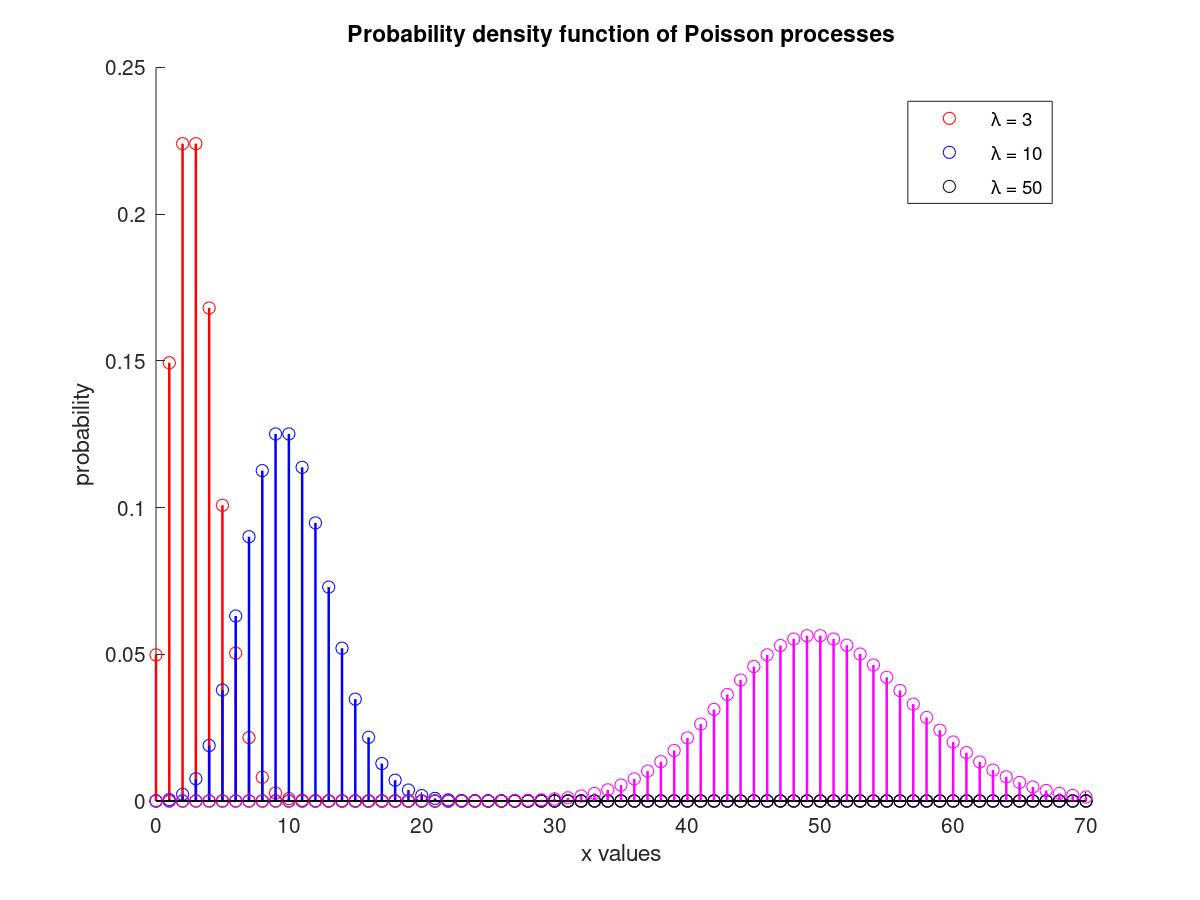
\includegraphics[width=\textwidth]{poissonA.jpg}
    \caption{Κατανομή \english{Poisson} με παραμέτρους $λ = {3, 10, 50}$}
    \label{fig:poissonA}
\end{figure}

Όπως βλέπουμε, η διαφορά μεταξύ των τριών ΣΜΜ, είναι ότι το κέντρο τους μετατοπίζεται ανάλογα με την παράμετρο λ (αφού αυτή είναι η μέση τιμή) και αφού και η διασπορά είναι λ, το εύρος της καμπύλης αυξάνεται όσο αυξάνουμε το λ.

\subsection*{Β)}

Οι τιμές που υπολογίζουμε για την μέση τιμή και την διακύμανση είναι $30$, γεγονός που το περιμέναμε, αφού στην κατανομή Poisson η μέση τιμή και η διακύμανση ισούνται με $30$.

\subsection*{Γ)}

Η υπέρθεση των κατανομών φαίνεται παρακάτω στο Σχήμα \ref{fig:poisson_conv}.

\begin{figure}
    \centering
    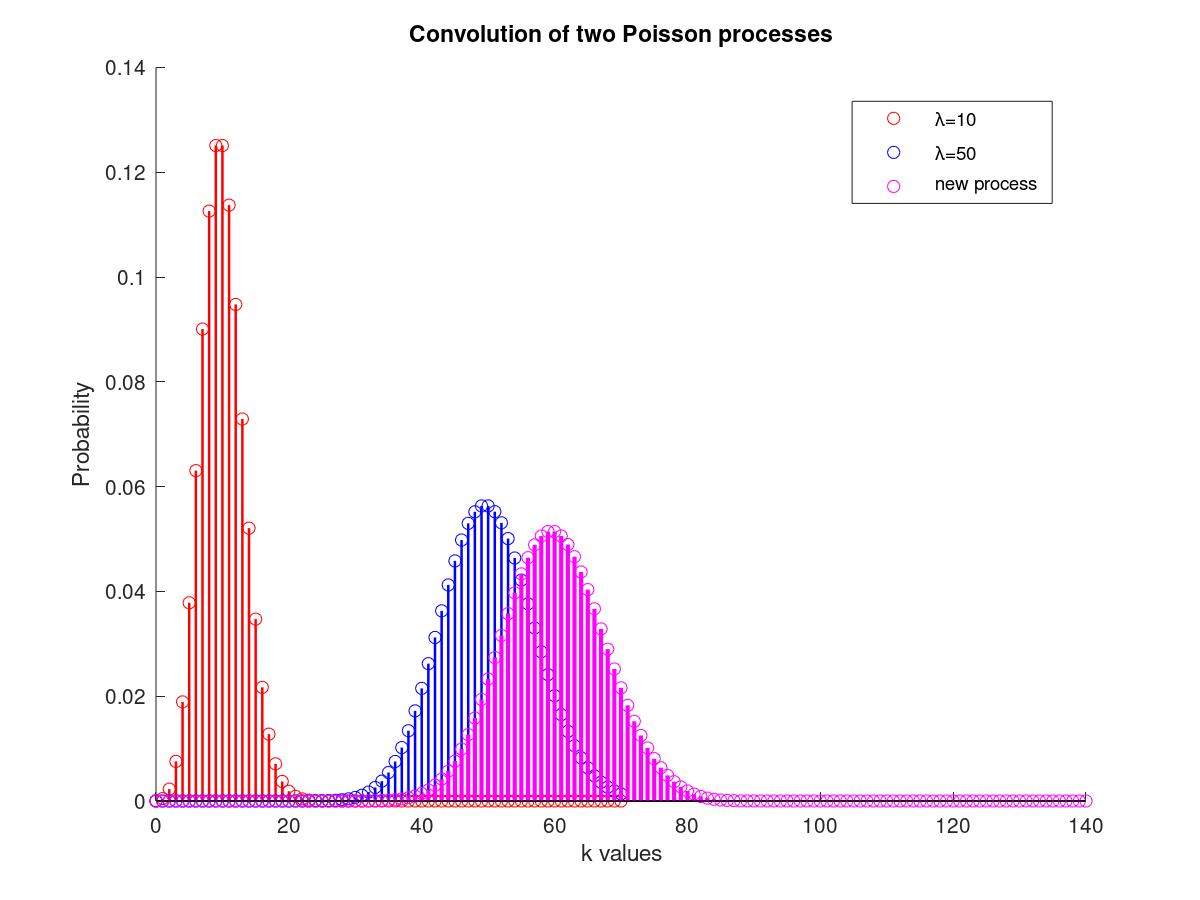
\includegraphics[width=\textwidth]{poisson_conv.jpg}
    \caption{Κατανομή \english{Poisson} με παραμέτρο  $λ = 50$, κατανομή με $λ = 10$ και η συνέλιξη τους.}
    \label{fig:poisson_conv}
\end{figure}


Η κατανομή που προέκυψε είναι και αυτή \english{Poisson} με $λ = 60$, δηλαδή η συνέλιξη των κατανομών \english{Poisson} με $λ = 50$ και $λ = 10$ μας οδήγησε σε μια κατανομή \english{Poisson} με $λ = 60$. H απαραίτητη προϋπόθεση για να συμβεί αυτό, είναι να είναι και οι δύο κατανομές \english{Poisson}.

\subsection*{Δ)}


Σύμφωνα με το οριοακό θεώρημα \english{Possion}, αν το όριο μιας όταν οι παράμετροι $n$ και $p_n$ είναι αρκετά μεγάλοι, και το γινόμενο τους συγκλίνει σε έναν αριθμό $λ$, δηλαδή $np_n = λ$, τότε η διωνημική οριακά γίνεται κατανομή \english{Poisson}. Τα αποτελέσματα φαίνονται στο Σχήμα \ref{fig:binom_to_poisson}. Όπως βλέπουμε, το $n$ στην πρώτη περίπτωση είναι πολύ μικρό και έτσι το τελικό αποτέλεσμα δεν μοίαζει με την \english{Poisson}, όπως θα περιμέναμε.

\begin{figure}
    \centering
    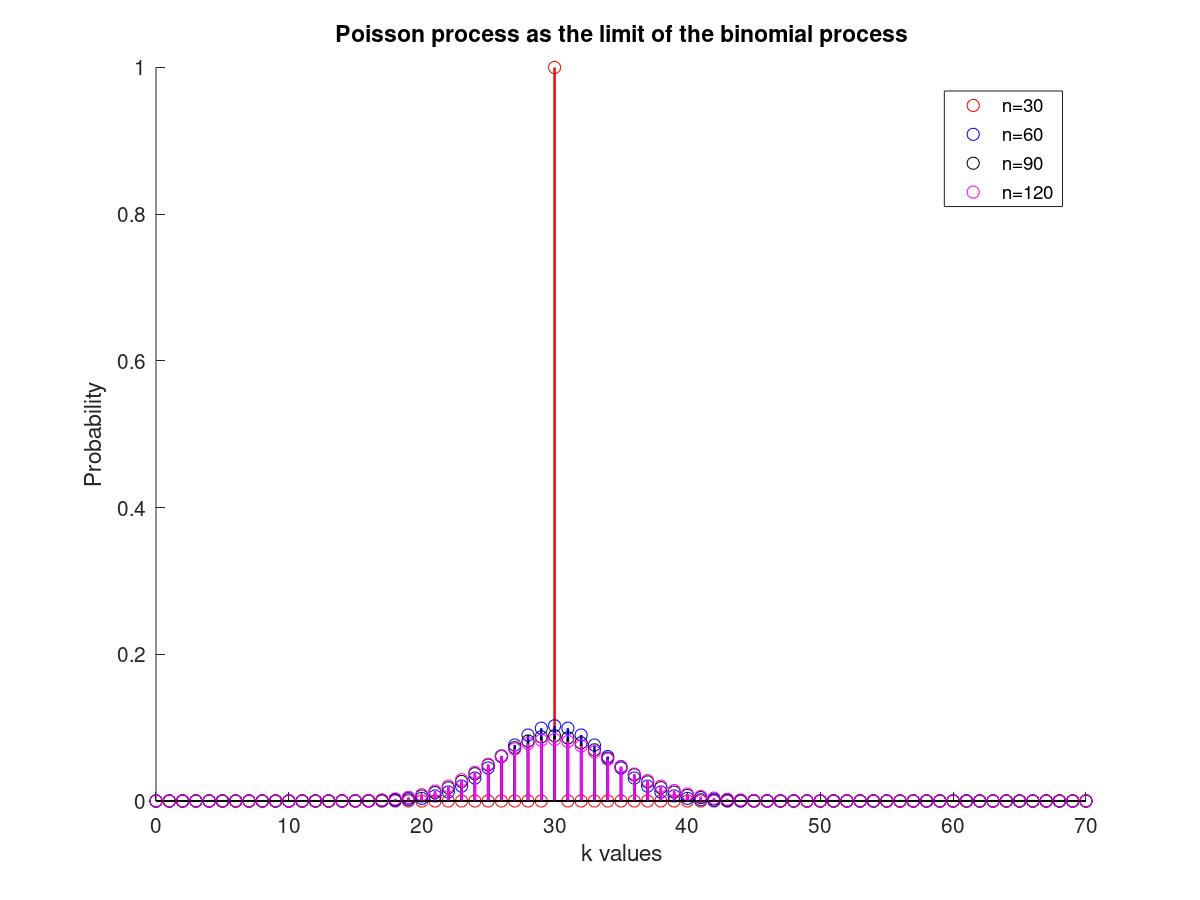
\includegraphics[width=\textwidth]{binom_to_poisson.jpg}
    \caption{Διωνυμικές κατανομές με $n = {30, 50, 90, 120}$}
    \label{fig:binom_to_poisson}
\end{figure}

\section*{Εκθετική κατανομή}

\subsection*{Α)}

Η σππ των εκθετικών κατανομών φαίνεται στο Σχήμα \ref{fig:exponential}.

\begin{figure}
    \centering
    \includegraphics[width=\textwidth]{expnential.png}
    \caption{Εκθετικές κατανομές με $\frac{1}{λ} = {0.5, 1, 3}$}
    \label{fig:exponential}
\end{figure}

\subsection*{Β)}

Η σκπ των εκθετικών κατανομών φαίνεται στο Σχήμα \ref{fig:exponential_cdf}.

\begin{figure}
    \centering
    \includegraphics[width=\textwidth]{expnential_cdf.png}
    \caption{Εκθετικές κατανομές με $\frac{1}{λ} = {0.5, 1, 3}$}
    \label{fig:exponential}
\end{figure}

\subsection*{Γ)}

Για να υπολογίσουμε το $\Pr{(x > 30000)}$, χρησιμοποιούμε τον τύπο $\Pr{(x > 3000)} = 1 –   \Pr{(x \leq 30000)}$. 

Για να υπολογίσουμε το $\Pr{(x > 50000 | x > 20000)}$ έχουμε σύμφωνα με τον τύπο της δεσμευμένης πιθανότητας:

\begin{equation*}
    \Pr{(x > 50000 | x > 20000)} = \frac{\Pr{(x > 50000 \cap x > 20000)}}{\Pr{(x > 20000)}} = \frac{\Pr{(x > 50000)}}{1 - \Pr{(x \leq 20000)}} = \frac{1 - \Pr{(x \leq 50000)}}{1 - \Pr(x \leq 20000)}
\end{equation*}

\end{document}
Παρατηρούμε ότι οι δύο πιθανότητες είναι και οι δύο ίσες με $0.88692$. Αυτό συμβαίνει λόγω την ιδιότητα έλλειψης μνήμης που έχει η εκθετική κατανομή. Πιο συγκεκριμένα σύμφωνα με τον τύπο της εκθετικής κατανομής, από την προτελευταία ισότητα της εξίσωσης μας και δεδομένου ότι η σκπ της εκθετικής είναι $e^{-λt}$, έχουμε $\frac{e^{-50000λ}}{e^{-20000λ}} = e^{{-20000λ}}$.